%%%%%%%%%%%%%%%%%%%%%%%%%%%%%%%%%%%%%%%%%%%%%%%%%%%%%%%%%%%%%%%%%%%%%%%%%%%%%%%%
\section{Scenario 1: Both Hosts on Ethernet}
\label{sec:wifi_water}
\begin{figure}[H]
    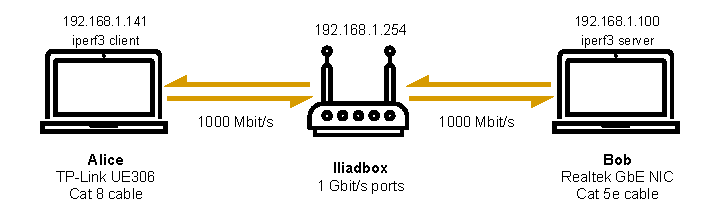
\includegraphics[width=0.90\linewidth]{images/wifi.drawio-4.pdf}
    \caption{Ethernet scenario}
    \label{fig:eth_to_eth_pic}
\end{figure}

\subsection{Scenario description}
For our first scenario, we set up the simplest network configuration: two hosts connected via Ethernet cables to the IliadBox router, which acted as a switch. Although this setup is straightforward, it is rarely used in everyday domestic environments. However, it remains widely prevalent in enterprise and corporate settings.

In this scenario, we had: Alice (\texttt{iperf3} client), IP: 192.168.1.141; Bob (\texttt{iperf3} server) with IP: 192.168.1.100.

\subsection{Computing the TMG}
In our setup, every device, adapter and port supports a maximum capacity of 1 Gbit/s. Therefore, we can assume the theoretical network capacity as $C = 1$ Gbit/s.

As discussed previously, when using an Ethernet connection in full-duplex mode, we need to account for the efficiency introduced by the various layers, namely Ethernet, IP and the transport layer protocol. We employed TCP, therefore, based on the previous theoretical computations (\ref{subsec:computations}), the TMG can be estimated as:
$$
\text{TMG} = \eta_{\text{TCPoFD}} \cdot C = 0.94 \cdot 1 \ \text{Gbit/s} = 940 \ \text{Mbit/s}
$$
This result reflects the expected goodput under ideal conditions, assuming no packet loss, latency, or other external disturbances. 
\subsection{Test results evaluation}
\begin{table}[htbp]
    \centering
    \caption{TCP Goodput from \texttt{iperf3} test (Mbit/s)}
    \label{tab:tcp-throughput-wired}
    \begin{tabular}{lrrrrc}
        \hline
        \textbf{Reverse flag} & \textbf{Avg} & \textbf{Median} & \textbf{Min} & \textbf{Max} & \textbf{Std Dev} \\
        \hline
        False & 937.6 & 938.0 & 937.0 & 938.0 & 0.49 \\
        True & 897.0 & 897.0 & 897.0 & 897.0 & 0.0 \\
        \hline
    \end{tabular}
    \end{table}

Table \ref{tab:tcp-throughput-wired} summarizes the \texttt{iperf3} test results for standard and reverse transmission modes.

In standard mode (reverse = False), the average goodput is 937.6 Mbit/s, with a median of 938.0 Mbit/s. The minimum (937.0 Mbit/s) and maximum (938.0 Mbit/s) values are close, resulting in a low standard deviation (0.49 Mbit/s), indicating stable performance. In reverse mode (reverse = True), the goodput remains constant at 897.0 Mbit/s, with zero variance, showing slightly lower yet stable performance. This difference may stem from transmission directionality or hardware handling.

Both configurations performed efficiently, with results close to the theoretical maximum goodput (950 Mbit/s).

By analyzing one of the PCAP files captured by the Python script, we can observe the overall behavior of the Ethernet scenario.

\begin{figure}[H]
    \centering
    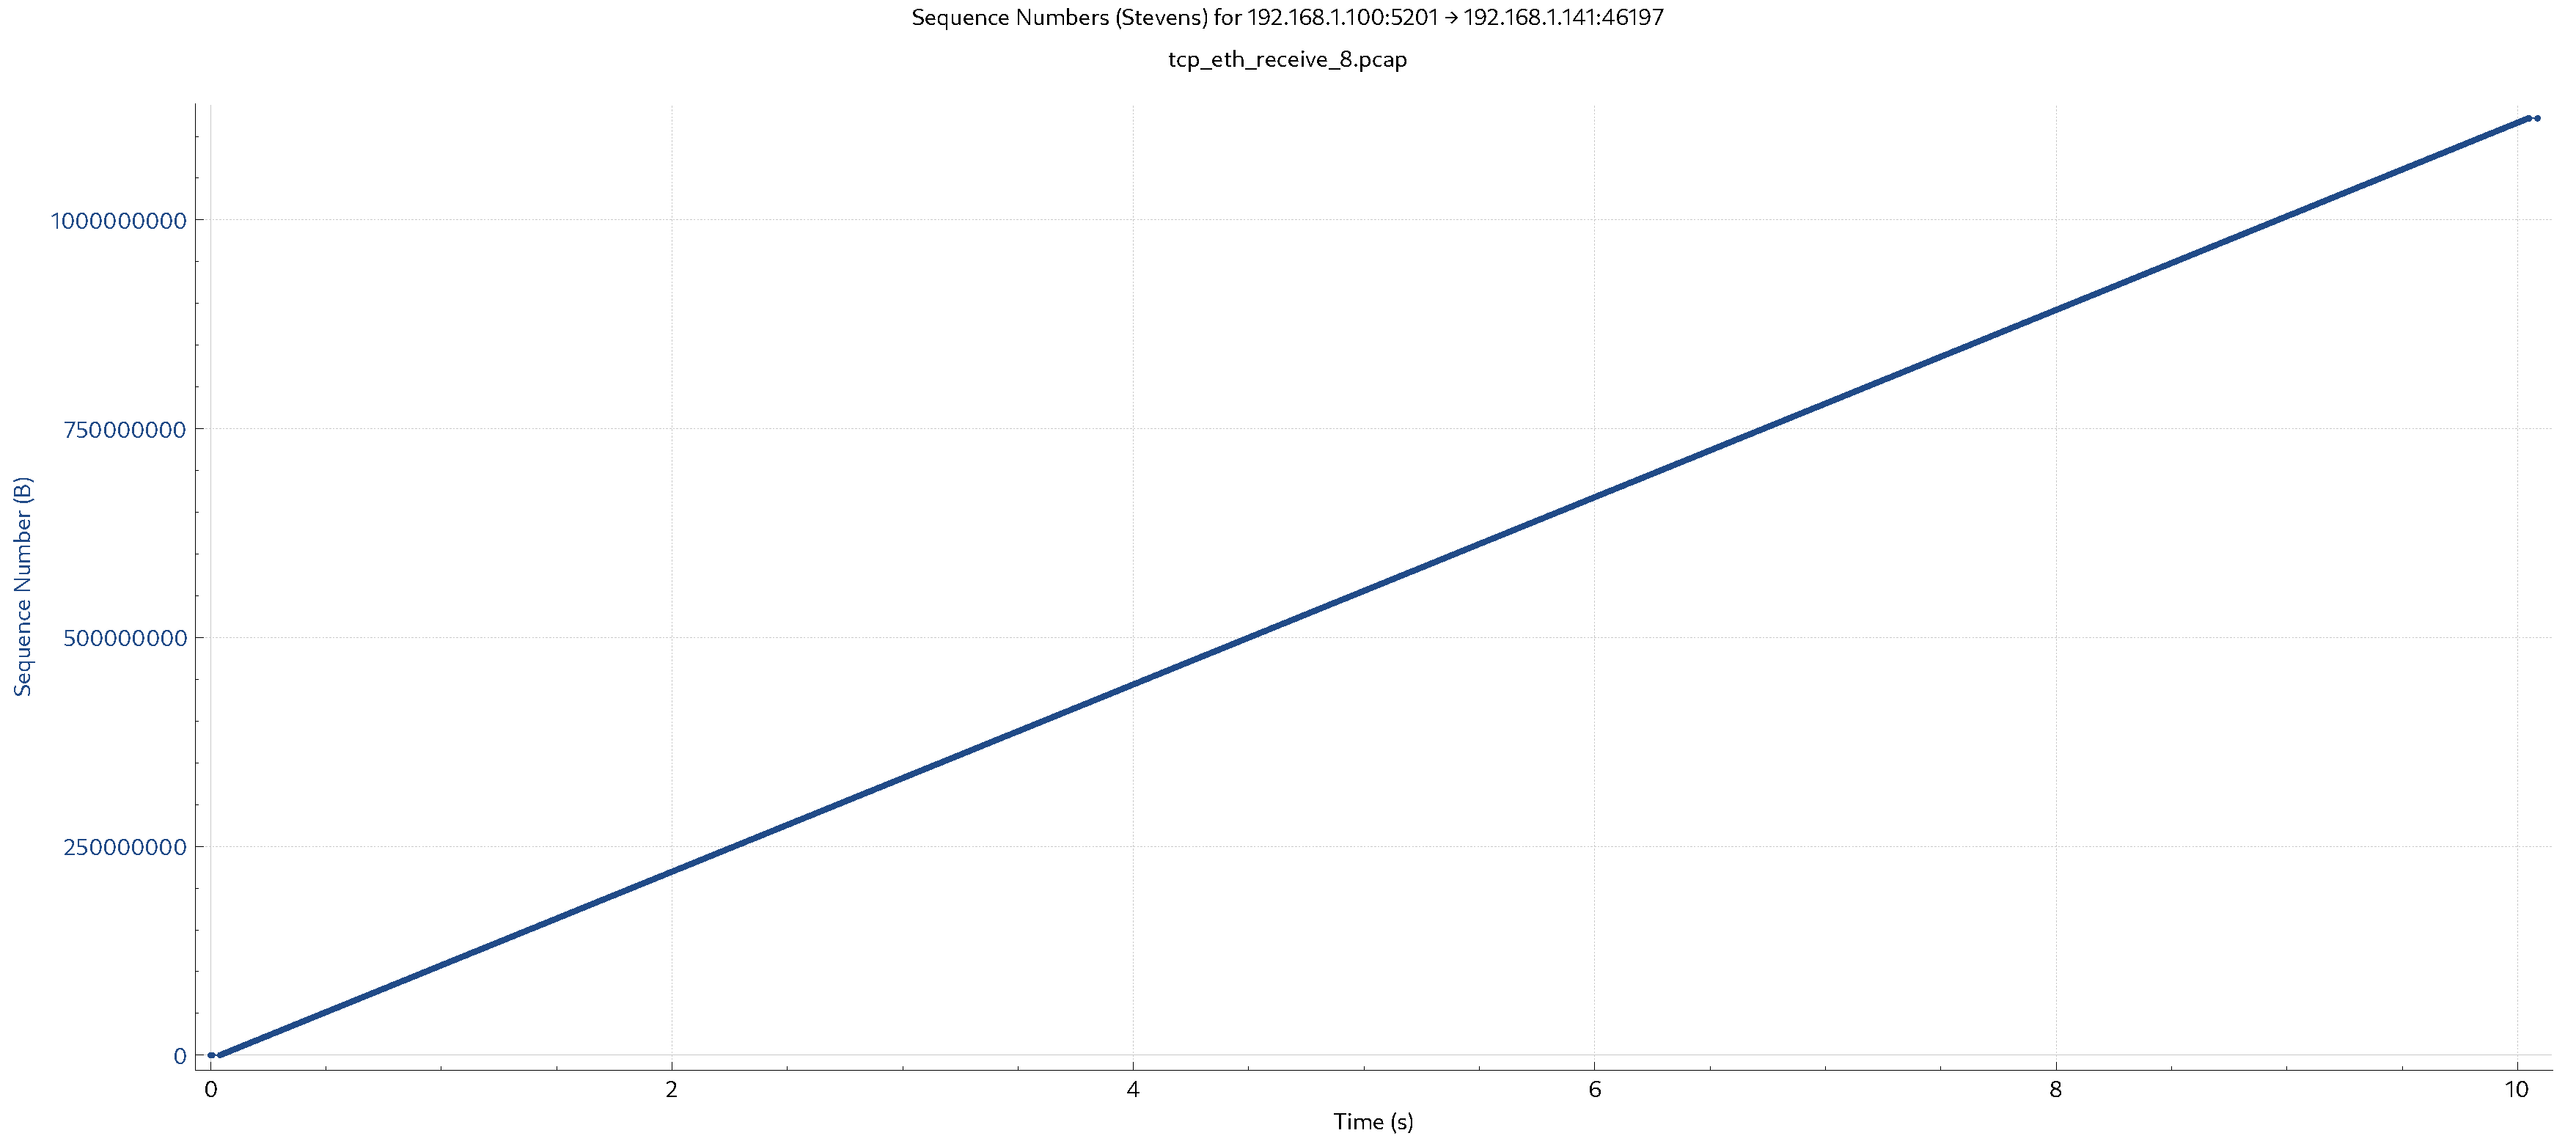
\includegraphics[width=0.75\linewidth]{SeqNumberEth.pdf}
    \caption{Sequence Numbers (Stevens), reverse flag set to True}
    \label{fig:enter-label}
\end{figure}


Looking at the graph that represents the sequence numbers of packets sent from the server (192.168.1.100) to the client (192.168.1.141) - which are the packets received when the reverse flag is enabled in \texttt{iperf3} - we notice that the graph forms a straight line. This indicates that the transmission occurred smoothly, without any retransmissions, and that the throughput remained consistent throughout the test.
We also plotted goodput computed by Wireshark.
\begin{figure}[H]
    \centering
    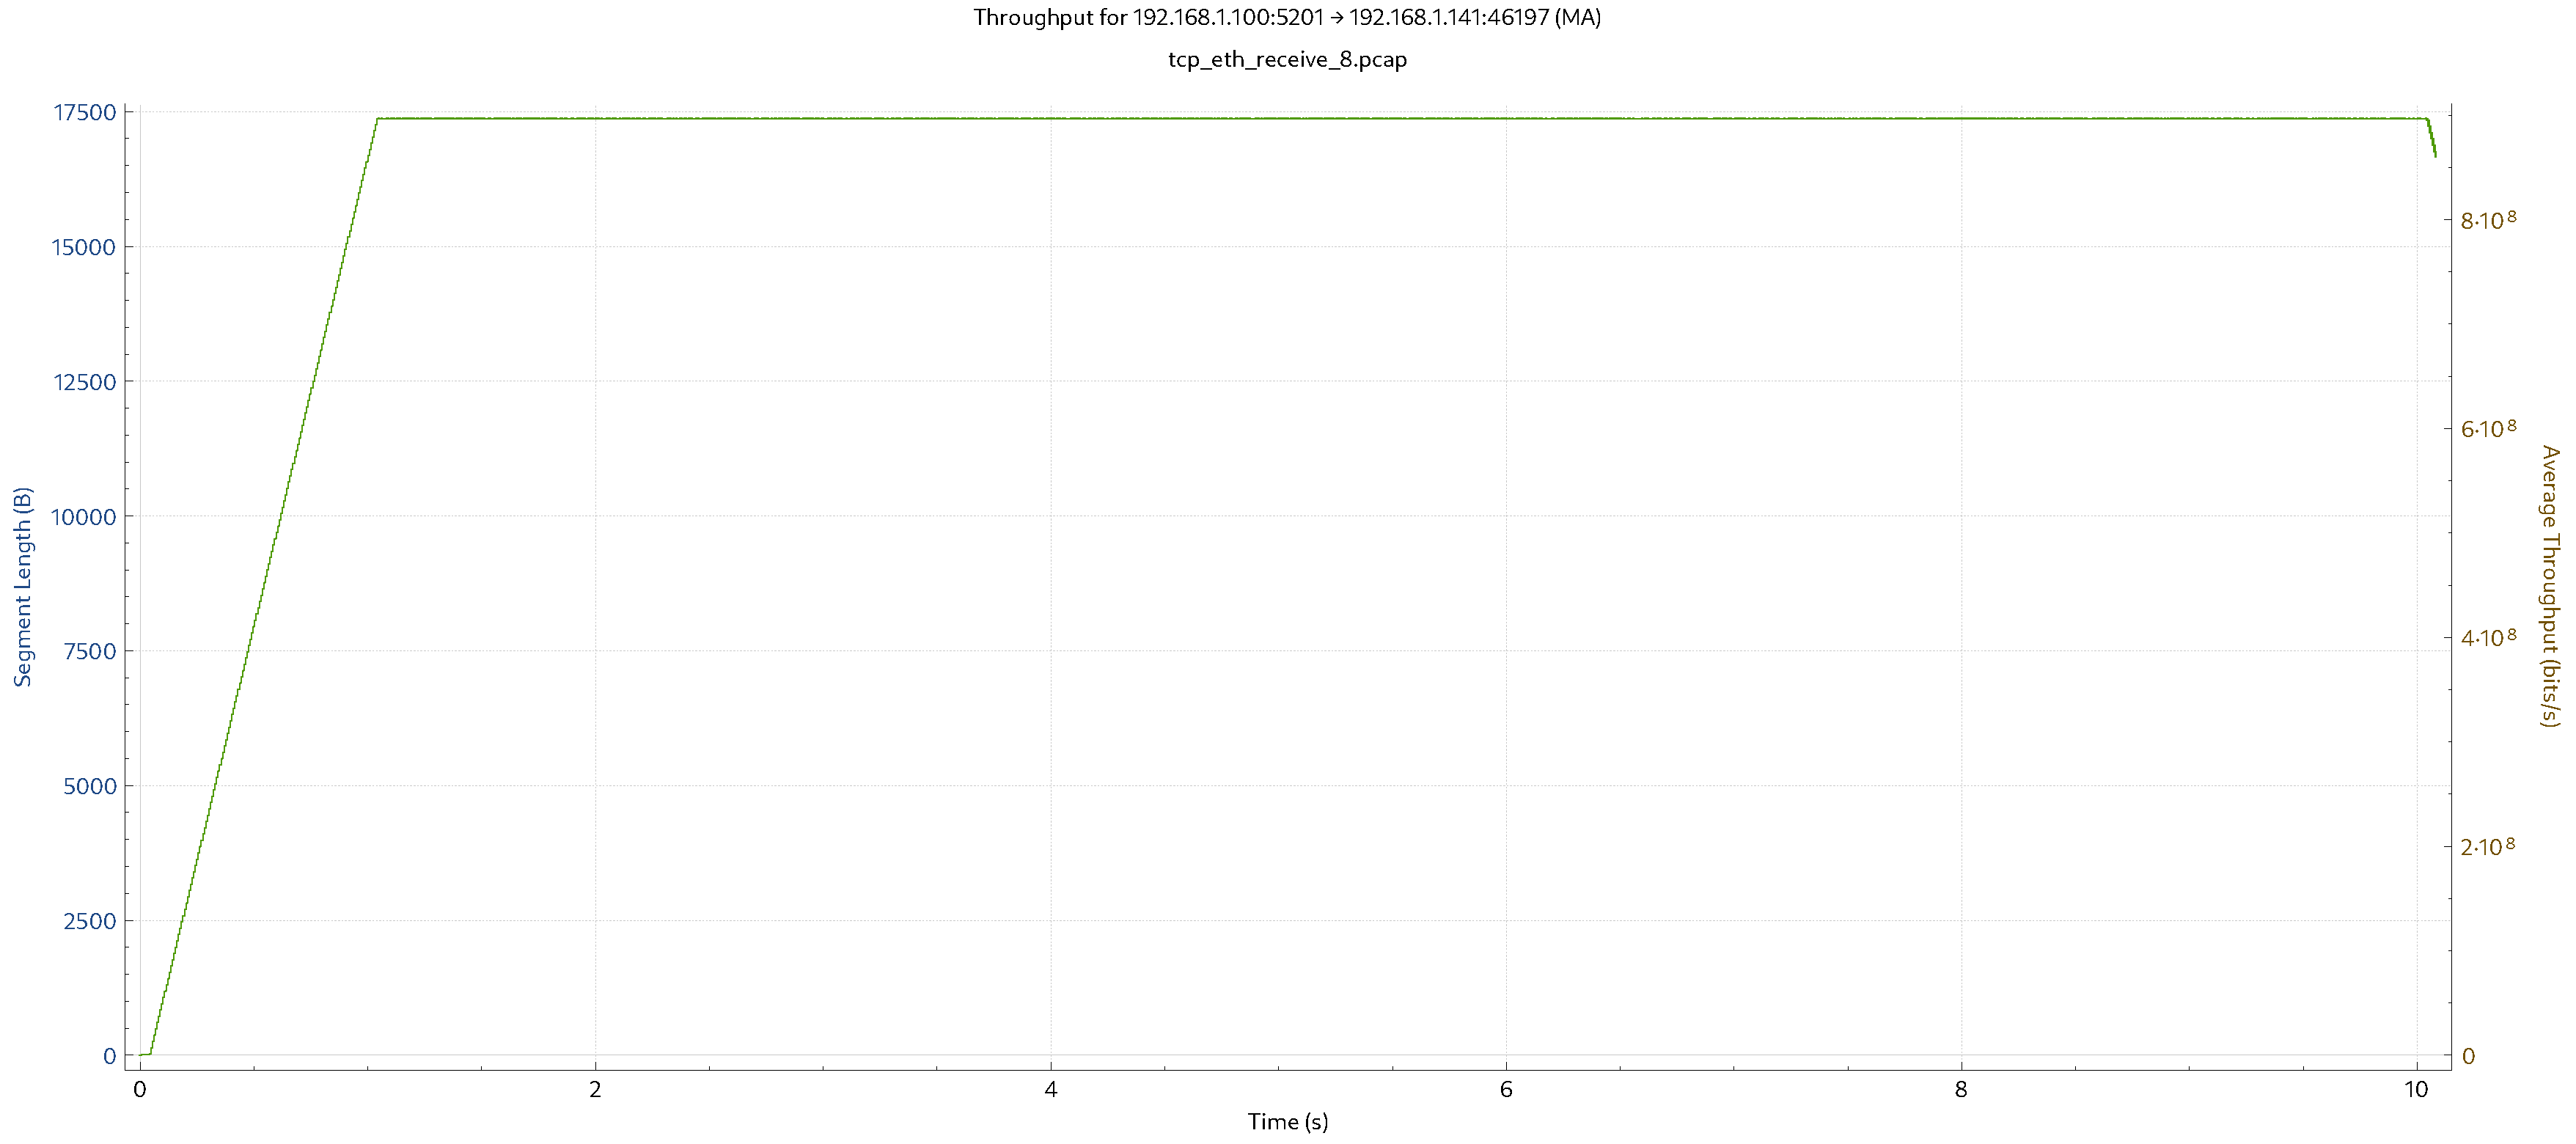
\includegraphics[width=0.75\linewidth]{GoodputEth.pdf}
    \caption{Goodput (MA) on the receiver side, reverse flag set to True}
    \label{fig:enter-label}
\end{figure}
It is important to note that we selected the "Goodput" option when generating the graph instead of "Throughput." 

However, we are unsure if Wireshark correctly differentiates between the two because both graphs appear identical.
